% This paper tries to present the thermodynamic point of view for studying the transportation system. To show the universe of this contribution, a general transportation model is used instead of the previous linear one.

% This new point of view is to analogize the transportation system to the thermodynamic system. The fundamental pair of correspondent concepts are the vehicle and the energy. The principles are introduced as well.

% preprint format
\documentclass[preprint,authoryear,12pt]{elsarticle}
% final format
% \documentclass[final,authoryear,5p,times,twocolumn]{elsarticle}
% \journal{}

% postScript packages and setting
\usepackage{graphicx}
\usepackage{ifpdf}
\ifpdf
\DeclareGraphicsExtensions{.pdf,.jpeg,.png}
\usepackage[bookmarks=true,colorlinks=true]{hyperref}
\else
\DeclareGraphicsExtensions{.eps}
\usepackage[bookmarks=true,colorlinks=true,dvipdfmx]{hyperref}
\fi
\usepackage{subfigure}

% mathematic packages and settings
\usepackage{amsmath}
\usepackage{amssymb}
\usepackage{amsthm}
\renewcommand{\vec}[1]{\mbox{\boldmath$#1$}}
\newcommand{\mat}[1]{\mbox{\boldmath$#1$}}
\newcommand{\unit}[1]{\,\mathrm{#1}}
\newtheorem{thm}{Theorem}
\newtheorem{lmm}{Lemma}
\newtheorem{ass}{Assumption}
\newtheorem{rmk}{Remark}
\newtheorem{dfn}{Definition}
\newtheorem{prpn}{Proposition}

\begin{document}

\begin{frontmatter}

\title{Thermodynamic Point of View for Urban\\ Transportation Network}
\author[SeT]{Huide Zhou\corref{cor}}
\ead{huide.zhou@utbm.fr}
\author[SeT]{Rachid Bouyekhf}
\ead{rachid.bouyekhf@utbm.fr}
\author[SeT]{Adbellah EL Moudni}
\ead{abdellah.el-moudni@utbm.fr}
\address[SeT]{Laboratoire Syst\`{e}mes et Transports (SeT),\\
Universit\'{e} de Technologie de Belfort-Montb\'{e}liard (UTBM)\\
Rue Thierry Mieg, 90010 Belfort Cedex, France}
\cortext[cor]{Corresponding author.}

\begin{abstract}
The paper endeavors to reply the following question: if we consider the vehicles as the abstract energy supplied to the transportation network, it is possible to analyze transportation systems from thermodynamic point of view? The strong motivation for this is that the study of transportation network is very hard. Consequently, if we can use thermodynamic concepts, which has been very well understood, we can effectively provide a new approach to study such systems.
% This paper presents a novel thermodynamic point of view to discover the nature of transportation systems. Indeed, if the vehicles are regarded as the energy supplied to the system, transportation systems are very similar with thermodynamic systems. Hence, the thermodynamic concepts can be introduced into the transportation context. In particular, transportation systems can have a similar notion of entropy to measure the system disorder. By taking the transportation entropy as the storage function, a dissipativity phenomenon is then presented to reduce the disorder and render the system better organized. Though this phenomenon doesn't exist naturally, it can be considered as the objective of traffic signal control. Furthermore, this paper also shows that the nominal situation in transportation systems is similar with the closed status in thermodynamic systems, and the equilibrium can be introduced into the transportation context to represent the state when all traffic lanes share the same occupancy.
This paper will show that, in certain circumstances, this idea works and certain thermodynamic concepts such as energy, temperature, thermal capacity, thermal equilibrium can have the corresponding notions in transportation context. In addition, it will be shown that, the most important thermodynamic notion, which is the entropy, can be also defined in order to measure the disorder of transportation systems. Then, by taking this entropy as the storage function, a dissipativity phenomenon is presented to reduce the disorder and render the system better organized. Finally, though the transportation network is always open, it will be shown that the nominal situation in transportation systems is similar with the closed status in thermodynamic ones.
\end{abstract}

\begin{keyword}
Transportation systems\sep thermodynamic systems \sep entropy\sep dissipativity theory.
\end{keyword}

\end{frontmatter}

\section{Introduction}

% Urban transportation is an essential part of the modern cities. Due to the rapid increase of traffic demands in recent decades, the congestion problem has become very frequent and led to serious economic and environment issues.

When we want to study the transportation network, we instantly meet computational difficulties that grow if the scale of the systems increases. This situation prevents us from obtaining a clear view of the influence of various factors on the behavior of the whole system. The analysis of transportation systems can be obtained in various ways, depending on the complexity of the problem, but the primary objective is to reduce computational efforts and to develop techniques that can be easily implemented on a computer, to allow automatic analysis of modeled systems. This situation has motivated many researchers to develop methods and techniques in order to circumvent difficulties involved in transportation systems. In particular, 
% To solve it, various approaches have been applied to understand the phenomenons in transportation systems. Among them,
the traffic flow theory has been the most widely used \citep{nathan_h_gartner_revised_2005}. This approach considers the vehicle movements as liquid flows, which matches the general impression of the traffic in modern cities. In addition, queueing theory has been applied to study the behavior of traffic flows near certain sections (e.g. traffic bottlenecks) where demand exceeds available capacity. The queuing and traffic flow theory can effectively describe the macroscopic traffic phenomenons and has led to several well-known traffic signal control strategies, like TRANSYT \citep{robertson_tansyt_1969,hale_traffic_2005}, SCOOT \citep{bretherton_r_d_scoot_1982}, TUC \citep{diakaki_multivariable_2002,papageorgiou_review_2003}, etc. Furthermore, from microscopic point of view, car-following models have been developed by taking human factors into account. In particular, car-following models examine the manner in which individual vehicles follow one another. This approach connects the microscopic behavior of individual vehicles and the macroscopic features of traffic flows. Another notable approach is the kinematic wave theory which studies the speed-density relationship from microscopic point of view \citep{zhang_kinematic_2002,jin_multicommodity_2004}. Its first-order approximation has led to the Cell Transmission Model (CTM) \citep{daganzo_cell_1995}, which has shown high accuracy in the simulation \citep{almasri_online_2005}. Hence, CTM has been used in traffic estimation \citep{CanudasdeWit2012,tampere_extended_2007} and traffic signal control \citep{Pohlmann2010}.
% Another well-known approach is the kinematic wave theory that shows the relationship between the traffic density and the traffic flow rate. Based on its first-order approximation, the Cell Transmission Model (CTM) has been further developed \citep{daganzo_cell_1995,flotterod_operational_2011}. The simulation of this model has shown results very close to the real systems. Benefit from its accuracy, CTM has been widely applied in the simulation \citep{Su2013}, the observer \citep{CanudasdeWit2012} and the traffic signal control \citep{Pohlmann2010}.
Besides, the applications of Petri nets (PNs) in modeling and control of transportation systems have been also conducted for over a decade \citep{ng_review_2013}. This tool is useful for analyzing performances and assisting intelligent traffic control.
% Another widely used model for the transportation system is the Petri-Net (PN) \citep{dotoli_urban_2006,ng_review_2013}, which works well with logic controllers.

In this paper, we propose another way to study transportation network which, to the best of  our knowledge,  has not been yet explored. Indeed, by regarding the  vehicles as the abstract energy supplied to the network, we show that certain  thermodynamic concepts can be applied to transportation systems. Among them, the most important notion is the entropy which measures system disorder and hence can be taken as a means to evaluate system performances.
% However, in our opinion, these existing works have done very little to explore the nature of the transportation system. They only focused on the superficial transportation behaviors and failed to show the fundamentals of the transportation phenomenon. Indeed, consider that the urban transportation system consists of the traffic lanes and the vehicles which can stay in the lanes or travel from one to another. This whole picture reminds us that the transportation system is very similar with the large-scale open thermodynamic system, which consists of connected subsystems (matters) and the energy that can be stored in subsystems or be transferred from one to another. The similarity encourages us to introduce thermodynamic concepts into transportation context to better understand the transportation phenomenons.

This paper is organized as follows: Section \ref{sec:concepts} will show the connections between the transportation system and the thermodynamic system. In particular, the basic concepts such as energy, temperature, thermal capacity can be introduced into the transportation context. Then, Section \ref{sec:entropy} will demonstrates that the transportation system can have a similar notion of entropy to measure the system disorder. By considering this new entropy notion as the storage function, a dissipativity law will be presented to reduce the disorder and hence render the system better organized. Finally, Section \ref{sec:nominal} will show that the nominal situation in transportation systems is similar with the closed status in thermodynamic ones.

\section{Basic Concepts and Conservation of Vehicles}\label{sec:concepts}

\subsection{Introduction to Transportation System}

The two fundamental elements of the urban transportation system are the traffic streets and the vehicles. The connected traffic streets provide a network within cities so that the vehicles can travel from their departure points to their destinations.

In details, a street is a linear traffic area connecting two separate points with a fixed length. When more than two streets meet in a single point, there will be a crossing area among these streets. These crossing areas and the connected streets compose the intersections \citep{papageorgiou_review_2003}. For example, Figure \ref{fig:int4leg} and Figure \ref{fig:int3leg} illustrate two common types of intersections, which connects 4 and 3 streets respectively.

\begin{figure}[ht]
  \centering
  \subfigure[Four streets]
  {\includegraphics{pics/int4leg}\label{fig:int4leg}}\quad
  \subfigure[Three streets]
  {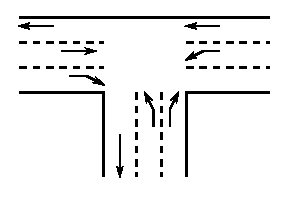
\includegraphics{pics/int3leg}\label{fig:int3leg}}
  \caption{Examples of intersections}
\end{figure}

Based on the directions of vehicles, a street can be further seperated into several traffic lanes. For example, the 4 streets in the intersection illustrated by Figure \ref{fig:int4leg} are all split into two lanes corresponding to two opposite directions. On the other hand, in Figure \ref{fig:int3leg}, the streets all consist of three lanes (Note that in this intersection, the lanes are split based on both the current and the potential directions of vehicles). A street may correspond to more than one traffic signals, but a lane can only correspond to one. Hence, the traffic lanes are more appropriate to be considered as the units of the traffic areas instead of the streets.
%Therefore, the transportation system is considered as the network of traffic lanes in this paper.
For each lane, the appropriate state variable is obviously the number of the vehicles within it, which, in this paper, is called the queue length of the traffic lane.

Now, observe that to accomplish the functionality of transportation, a vehicle need enter the transportation network from its departure point, travel from one lane to another until leaving the system at its destination. This is the fundamental of the transportation system. Hence, the dynamic of the system is reflected by the movements of vehicles. By applying the traffic flow theory \citep{nathan_h_gartner_revised_2005}, these movements can be considered as traffic flows.

Consider a transportation network including $n$ traffic lanes, $n>0$. Figure \ref{fig:flows} illustrates all traffic flows related with the lane $i$, $i\in\{1,\cdots,n\}$. $x_i$ is the queue length of lane $i$; the flow $r_i$ denotes the vehicles entering the lane $i$ from the outside; the flow $\sigma_{i,j}$ (resp, $\sigma_{j,i}$), $j\neq i$, $j\in\{1,\cdots,n\}$, represents the vehicles travel from the lane $j$ (resp, $i$) queue to the lane $i$ (resp, $j$); the flow $d_{i}$ is the output flow denoting the vehicles which leave the transportation system from the lane $i$.

\begin{figure}[ht]
  \centering
  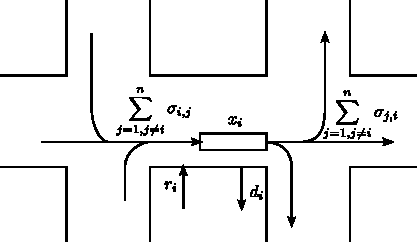
\includegraphics{pics/flows}
  \caption{The traffic flows related with the lane $i$}
  \label{fig:flows}
\end{figure}

To describe the dynamic of the transportation system from discrete-time approach, the change of the queue length $x_i$ during the interval $k$, $k\in\mathbb{N}$, is given by
\begin{equation}\label{equ:mdl_gnl_lane}
\Delta x_i(k) = l_i(k)+r_i(k)-d_i(k)
\end{equation}
where $l_i$ is the sum of all exchange flows related with lane $i$, which means
\begin{equation}\label{equ:exchange_vehicle}
 l_i(k)=\sum_{j=1,j\neq i}^{n}(\sigma_{i,j}(k)-\sigma_{j,i}(k))
\end{equation}
Equivalently, in vector form, the transportation system can be represented by the following state-space difference equation
\begin{equation}\label{equ:mdl_gnl}
\vec{x}(k+1)=\vec{x}(k)+\vec{l}(k)+\vec{r}(k)-\vec{d}(k),\quad \forall k\in\mathbb{N}
\end{equation}
where $\vec{x}=[x_1,\cdots,x_n]^T$, $\vec{l}=[l_1,\cdots,l_n]^T$, $\vec{r}=[r_1,\cdots,r_n]^T$, $\vec{d}=[d_1,\cdots,d_n]^T$, and $x_i(k)$ is the queue length of lane $i$ at the beginning of the interval $k$.

It is important to note that without any specific assumption, \eqref{equ:mdl_gnl} is a general model, which fits any kind of transportation system in any circumstance. Based on this general model, we will explore the nature of transportation system from thermodynamic point of view in the sequel.

\subsection{Introduction to Thermodynamic System}

The fundamental concept for analyzing the large-scale thermodynamic systems is the concept of energy. Indeed, assume that a matter with an unique temperature is called a subsystem, the thermodynamic system consists of a set of connected subsystems. Each of them can store certain quantities of energy and exchange energy with other subsystems.
% which can store certain quantities of energy and are connected so that the energy can be transferred among them.
Let the energy stored by the subsystems be their state variables. The dynamic of these states is determined by the energy flows between the subsystems and their surroundings.
% In this paper, the work done by either the system or the environment is not concerned, hence the energy flows have only the form of heat which is driven by the temperature differences.

Recently, \citet{haddad_thermodynamic_2005} presented a discrete-time model for the large scale open thermodynamic system. Now, consider a thermodynamic system including $n$ subsystems. As shown in Figure \ref{fig:Ther_Sys}, the $i$th subsystem is denoted by $\Psi_i$, $i\in \{1,\cdots,n\}$, and its stored energy is denoted by $E_i$. Let $E_i^*>0$ be the thermal capacity of $\Psi_i$, then the temperature of $\Psi_i$ is given by
\begin{equation}\label{equ:temperature}
    T_i= {E_i}/{E^*_i}
\end{equation}

\begin{figure}[ht]
  % Requires \usepackage{graphicx}
  \centering
  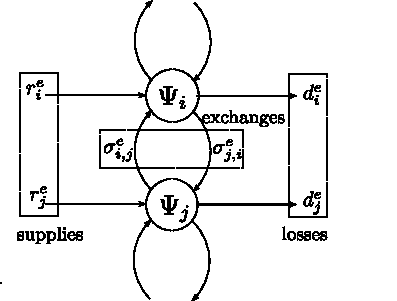
\includegraphics{pics/HModel}
  \caption{Thermodynamic system}
  \label{fig:Ther_Sys}
\end{figure}

In Figure \ref{fig:Ther_Sys}, the energy flow supplied by the outside to $i$th subsystem is denoted by $r^e_i$. The flow $\sigma^e_{i,j}$ (resp, $\sigma^e_{j,i}$), $i\neq j$, $i,j\in \{1,\cdots,n\}$, represents the transmission of energy from the $j$th (resp, $i$th) subsystem to the $i$th (resp, $j$th) subsystem. The flow $d^e_i$, $i\in \{1,\cdots,n\}$, represents the energy loss from the $i$th subsystem to the outside of the system. By combining the input, exchange and output energy flows, the dynamic of the energy $E_i$ stored by $\Psi_i$ can be given by
\begin{equation}\label{equ:Ther_Model_SubSystem}
\Delta E_i(k) = \sum_{j=1,j\neq
i}^{n}(\sigma^e_{i,j}(k)-\sigma^e_{j,i}(k))+r^e_i(k)-d^e_i(k)
\end{equation}
which equivalently infers the state-space model of the thermodynamic system
\begin{equation}\label{equ:Ther_Model}
    \vec{E}(k+1)=\vec{E}(k)+\vec{l}^e(k)+\vec{r}^e(k)-\vec{d}^e(k)
\end{equation}
where $\vec{E}(k)=[E_1(k),\cdots,E_n(k)]^T$ is the vector of the energy stored by all subsystems at the beginning of $k$th interval, $\vec{r}^e=[r^e_1,\cdots,r^e_n]^T$, $\vec{d}^e=[d^e_{1},\cdots,d^e_{n}]^T$, and $\vec{l}^e=[l^e_1,\cdots,l^e_n]^T$ represents all exchange flows such that
\begin{equation*}
l^e_i = \sum_{j=1,j\neq i}^{n}
        (\sigma^e_{i,j}-\sigma^e_{j,i}),
\; i\in \{1,\cdots,n\}
\end{equation*}

\subsection{Correspondences of Basic Concepts}

Now, by comparing the transportation model \eqref{equ:mdl_gnl} and the thermodynamic model \eqref{equ:Ther_Model}, it is clear that these two systems have many common aspects. In particular, the vehicles perform very similarly as the energy does in the thermodynamic system. Hence, the vehicles can be considered as the transportation ``energy''. Based on this fundamental correspondence, the thermodynamic concepts can be introduced into the transportation context.

Indeed, each traffic lane can contain certain amount of vehicles. The vehicles move between the connected lanes or between a lane and the outside. Obviously, the lanes are like the subsystems in the thermodynamic context, which store energy and exchange energy with their surroundings. Hence, the traffic lane is the corresponding notion of the thermodynamic subsystem and the queue lengths $x_i$ correspond to the energy stored in subsystems $E_i$, $i\in\{1,\cdots,n\}$.

The temperature is also an important thermodynamic concept. For finding its correspondence in transportation context, the corresponding notion of the thermal capacity should be firstly found. Since the lengths of traffic lanes are fixed, hence there exists a maximal capacity for each lane to contain vehicles. Let $x_i^*$, $i\in\{1,\cdots,n\}$, be the capacity of the lane $i$. It is not difficult to observe that the appropriate corresponding notion of the thermal capacity $E_i^*$ is the lane capacity $x_i^*$. Furthermore, we can define the occupancy of a lane as the proportion of the queue length to the capacity, which is given by
\begin{equation}\label{equ:occupancy}
f_i = \frac{x_i}{x_i^*},\quad i\in\{1,\cdots,n\}
\end{equation}
Compared with the equation \eqref{equ:temperature}, the occupancies $f_i$ obviously correspond to the temperatures $T_i$, $i\in\{1,\cdots,n\}$.

In summary, Table \ref{tab:notions} lists the correspondences of the basic concepts between thermodynamic and transportation systems. This analogy will provide us the opportunity to introduce thermodynamic principles into transportation context as well.

\begin{table}[ht]
\centering \caption{Correspondence of basic concepts}
\label{tab:notions}
\begin{tabular}{cc}
  \hline
  % after \\: \hline or \cline{col1-col2} \cline{col3-col4} ...
  Thermodynamic Concepts & Transportation Concepts \\
  \hline
  energy & vehicle \\
  subsystem & traffic lane \\
  energy stored in subsystems & queue lengths \\
  thermal capacity & lane capacity \\
  temperature & occupancy \\
  \hline
\end{tabular}
\end{table}

\subsection{Conservation of Vehicle (First Principle)}

The first law of thermodynamics, called the conservation of energy \citep{cengel_thermodynamics:_2001}, indicates that the energy can not be created or destroyed, it can only change forms or be transferred. Specially, the change of the energy stored in any thermodynamic system equals exactly the amount of the net energy exchange with its surroundings.

This principle also holds for the transportation system, because the change of  vehicles within a  system equals exactly the amount of the net traffic flows between the system and the outside. To show this principle more clearly, the following theorem is presented and proved based on the general transportation model \eqref{equ:mdl_gnl}.

\begin{thm}\label{thm:conservation}
Let $\vec{\epsilon} \triangleq [1,\cdots,1]^T$ be the vector whose all components are equal to $1$, and 
 define
\begin{equation}\label{equ:total_vehicle}
U \triangleq \vec{\epsilon}^T\vec{x}
\end{equation}
as the total number of the vehicles within the transportation network. Let
\begin{equation}\label{equ:all_io}
Q \triangleq \vec{\epsilon}^T(\vec{r}-\vec{d})
\end{equation}
be the number of the net vehicles moving from the outside into the transportation network. Then, the following statement holds $\forall k\in\mathbb{N}$
\begin{equation}\label{equ:conservation}
\Delta U(k) = Q(k)
\end{equation}
where $\Delta U(k)=U(k+1)-U(k)$.
\end{thm}
\begin{proof}
From \eqref{equ:mdl_gnl}, we have
\begin{align*}
U(k+1) &= \vec{\epsilon}^T\vec{x}(k+1)\\
       &=
\vec{\epsilon}^T\vec{x}(k)+\vec{\epsilon}^T\vec{l}(k)+\vec{\epsilon}
^T(\vec{r}(k)-\vec{d}(k))\\
       &= U(k)+\vec{\epsilon}^T\vec{l}(k)+Q(k)
\end{align*}
It follows
$$\Delta U(k)-Q(k) = \vec{\epsilon}^T\vec{l}$$
Now, observe that $\vec{\epsilon}^T\vec{l}(k) =\displaystyle \sum_{j=1}^{n} l_i(k)$ and since $l_i(k)=\displaystyle\sum_{j=1,j\neq i}^{n}(\sigma_{i,j}(k)-\sigma_{j,i}(k))$ in view of \eqref{equ:exchange_vehicle}, it follows
% Hence, \eqref{equ:conservation} is equivalent to
% $$\vec{\epsilon}^T\vec{l}(k)=0,\quad \forall k\in\mathbb{N}$$
% Now, because
% $$l_i(k)=\sum_{j=1,j\neq i}^{n}(\sigma_{i,j}(k)-\sigma_{j,i}(k))$$
% it infers that
\begin{align*}
\vec{\epsilon}^T\vec{l}(k)
    &= \sum_{i=1}^n (\sum_{j=1,j\neq i}^{n} \sigma_{i,j}(k)
       -\sum_{j=1,j\neq i}^{n} \sigma_{j,i}(k))\\
    &= \sum_{i=1}^n \sum_{j=1,j\neq i}^{n} \sigma_{i,j}(k)
       -\sum_{i=1}^n \sum_{j=1,j\neq i}^{n} \sigma_{j,i}(k)\\
    &= \sum_{i=1}^n \sum_{j=1,j\neq i}^{n} \sigma_{i,j}(k)
       -\sum_{j=1}^n \sum_{i=1,i\neq j}^{n} \sigma_{j,i}(k)\\
    &= 0
\end{align*}
which is the desired result.
\end{proof}

This theorem indicates that the total vehicles in the transportation system depends only on the traffic flows between the system and the outside, the exchange flows between different lanes can not change the total number of the vehicles within the network. Furthermore,\eqref{equ:conservation} implies
\begin{equation}\label{equ:conservation_ex}
U(k_2) = U(k_1)+\sum_{k=k_1}^{k_2-1}Q(k)
\end{equation}
for any $k_1,k_2\in\mathbb{N}$, $k_2>k_1$. Hence, according to \citep{willems_dissipative_1972-1}, the conservation of vehicles also implies that the transportation system \eqref{equ:mdl_gnl} is lossless with respect to the storage function \eqref{equ:total_vehicle} and the supply function \eqref{equ:all_io}.

\section{Transportation Entropy and Dissipativity}\label{sec:entropy}

\subsection{Second Law of Thermodynamics}

In the thermodynamic system, the directions and the quantities of the energy movements must follow some specific rules. For example, without heating equipment, a hot beverage will definitely become cooler in a cold room. Consequently, the energy can not move from cold air to the hot beverage but in the opposite direction. These phenomenons are consistent with the second law of thermodynamics (Clausius statement, \citet{clausius_mechanical_1867}):
\begin{quotation}
\it Heat can never pass from a colder to a warmer body without some other change, connected therewith, occurring at the same time.
\end{quotation}

This principle is usually connected with a special concept of \textbf{entropy}. The second law of thermodynamics can be also described by the way how the entropy of thermodynamic system changes.
% For example, the heat can be transferred from hotter objects to colder ones, but it can never go in the opposite direction. Certain phenomenons have been studied and generated the second law of thermodynamics \citep{cengel_thermodynamics:_2001}, which introduced a special concept.
In particular, Clausius proposed that the increase of the system entropy due to the input energy $Q$ from the environment is $Q/T^a$, where $T^a$ is the absolute temperature at the sport where the energy transmission happens \citep{clausius_mechanical_1867}. However, for any thermodynamic system, the actual increase of entropy is bigger than or equals to the one supplied by the environment. In other words, any thermodynamic system is creating entropy itself. This phenomenon can be presented by the following inequality
\begin{equation}\label{equ:clausius_ther_gnl}
\Delta \psi \ge \int\frac{dQ}{T^a}
\end{equation}
or its discrete-time version \citep{haddad_thermodynamic_2005}
\begin{equation}\label{equ:clausius_ther}
\psi(k+1) \ge \psi(k)+\sum_{i=1}^{n}\frac{Q_i(k)}{T^a_i(k+1)},
\forall k\in\mathbb{N}
\end{equation}
where $\psi$ is the entropy of the thermodynamic system, $Q_i(k)$ is the net energy that the $i$th subsystem absorbs from the outside during the interval $k$, and $T^a_i(k+1)$ is the absolute temperature of the $i$th subsystem at the end of interval $k$, $i\in\{1,\cdots,n\}$. \eqref{equ:clausius_ther_gnl} and \eqref{equ:clausius_ther} are also known as Clausius inequality.

 Furthermore, since the entropy is opposite to the capacity of the thermodynamic system to do useful work, it is also regarded as the measure of the system disorder \citep{balmakov_entropy_2001}. More precisely, bigger entropy indicates that the system is worse organized. Hence, the Clausius inequality also implies that the thermodynamic system always tends to become worse organized.

For the discrete-time thermodynamic model \eqref{equ:Ther_Model}, based on the Clausius inequality \eqref{equ:clausius_ther}, \citet{haddad_thermodynamic_2005} presented the formula of its entropy as follows
\begin{equation}
\psi(\vec{E}) \triangleq{\vec{E}^*}^T \ln
(a\vec{\epsilon}+\mat{P}_e\vec{E}) -\vec{\epsilon}^T\vec{E}^*\ln a
\label{equ:Ther_entropy}
\end{equation}
where $\psi(\vec{E})$ is the entropy, $\vec{E}^*=[E^*_1,\cdots,E^*_n]^T$, $a$ is a positive scalar which represents the difference between the absolute temperature and the temperature defined in \eqref{equ:temperature} so that $T^a_i=a+T_i$, $i\in\{1,\cdots,n\}$, and $\mat{P}_e$ is a diagonal matrix with diagonal elements $1/E^*_i$. Here, the logarithm of a vector is the vector of the logarithm of each component.

Note that this formula is identical with the Boltzmann entropy expression for statistical thermodynamics. Indeed, for any subsystem without phase transition, the entropies in different absolute temperatures ($T1$, $T2$) satisfy the following relationship \citep{cengel_thermodynamics:_2001}
\begin{equation}\label{equ:entropy_temperature}
\psi_i(T1)-\psi_i(T2)=E_i^* \ln \frac{T1}{T2},\quad \forall
i\in\{1,\cdots,n\}
\end{equation}
It is known that the absolute temperature of the $i$th subsystem equals $a+\frac{E_i}{E_i^*}$. Specially, when the subsystem stores no energy ($E_i=0$), its absolute temperature becomes $a$. Hence, \eqref{equ:entropy_temperature} implies
\begin{align}
\psi_i(E_i)&=\psi_i(0)+E_i^* \ln \frac{a+\frac{E_i}{E_i^*}}{a}
\nonumber\\
&=\psi_i(0)+E_i^* \ln (a+\frac{E_i}{E_i^*})-E_i^* \ln{a}
\label{equ:tmp_psi_1}
\end{align}
Now, according to the third law of thermodynamics, the entropy approaches zero when the stored energy approaches zero, which means
\begin{equation}\label{equ:entropy_zero}
\psi_i(0)=\lim_{E_i\rightarrow 0}\psi_i(E_i)=0
\end{equation}
Therefore, we have
\begin{equation}
\psi_i(E_i)=E_i^* \ln (a+\frac{E_i}{E_i^*})-E_i^* \ln{a}
\end{equation}
By summarizing all subsystems, the entropy of the whole system is given by
\begin{equation}
\psi(\vec{E})=\sum_{i=0}^n E_i^*\ln(a+\frac{E_i}{E_i^*})-E_i^*\ln a
\end{equation}
which infers the Haddad's formula of entropy \eqref{equ:Ther_entropy}.

Furthermore, since the entropy \eqref{equ:Ther_entropy} is not easy to apply in control issues, \citet{haddad_thermodynamic_2005} also introduced a dual notion to entropy, called ectropy, to measure the system order. The dual inequality to \eqref{equ:clausius_ther} is given by
\begin{equation}\label{equ:anti_clausius}
\phi(k+1)-\phi(k)\le \sum_{i=0}^n Q_i(k)T_i(k+1),
\forall k\in\mathbb{N}
\end{equation}
where $\phi$ is the ectropy of the thermodynamic system, $Q_i(k)T_i(k+1)$ is the input ectropy of $i$th subsystem supplied by the environment with the net input energy $Q_i(k)$, and $T_i(k+1)$ is the temperature of $i$th subsystem at the end of interval $k$. This inequality is also called anti-Clausius inequality, which, like Clausius inequality, is consistent with the second law of thermodynamics.

Anti-Clausius inequality indicates that in any circumstance, any thermodynamic system is destroying its ectropy so that the increase of the ectropy is always less than the one supplied from its surroundings. Opposite with the entropy, the ectropy measures the capacity of the system to do useful work, and bigger ectropy corresponds to better organization of the system.

For the discrete-time thermodynamic model \eqref{equ:Ther_Model}, based on the anti-Clausius inequality \eqref{equ:anti_clausius}, \citet{haddad_thermodynamic_2005} presented the formula of the ectropy as follows
\begin{align}
\phi(\vec{E})&\triangleq\frac{1}{2}\vec{E}^T \mat{P}_e \vec{E}
\label{equ:Ther_ectropy}
\end{align}

Contrary to the energy, the entropy and the ectropy are both non-conservative notions. Specially in the isolated system, the sum of energy always keeps constant, but the entropy tends to increase while the ectropy tends to decrease. Besides, it is important to note that the ectropy \eqref{equ:Ther_ectropy} has the form of Lyapunov function, which is more useful in control issues than the entropy.

\subsection{Transportation Entropy}
% The above section has analogized the transportation system to the thermodynamic system, which encourages us to introduce entropy concept into transportation context to be the evaluation of the system performance.
The correspondence between transportation systems and thermodynamic systems encourages us to introduce the entropy concept into transportation context in order to evaluate the system performances. However, the problem is that there is no natural principle in transportation context that corresponds to the second law of thermodynamics. As a matter of fact, the directions of vehicles are determined by the drivers, there is no such rule that the vehicles only move from more crowded lanes to less crowded ones. Hence, we can not introduce transportation entropy based on certain principles as it is defined in the thermodynamic context. However, Nevertheless, based on the correspondences of certain concepts, such as energy and temperature, we can still simply introduce the formulas in the thermodynamic system to present the transportation entropy as the measure of the system disorder.

To do this, the significations of orders in these two systems must be firstly compared. Indeed, in thermodynamic context, higher order means higher capacity to do useful work, which is related with bigger temperature differences between subsystems. For example, in a thermodynamic system including two subsystems, if more energy concentrates on one single subsystem to generate bigger temperature difference, the quantity of the potential energy movements is bigger, which means that the system can generate more useful work. In this case, the system is regarded as better organized and has higher order. But on the converse, the bigger differences between the occupancies correspond to lower order in transportation context. Indeed, for a general transportation network, if more vehicles concentrate in only a few lanes, it has bigger probability to generate congestions in these lanes and the other lanes are wasted. In this case, the system is regarded as worse organized and has lower order.

Moreover, the energy input to the thermodynamic system brings more capacity to do useful work, which increases the order. However, in transportation context, the vehicle input brings more potential opportunity to generate congestions, which decrease the order. For an isolated thermodynamic system without energy input, the disorder (entropy) can only increase until it reaches equilibrium. On the converse, if, at a certain moment, the transportation system has no vehicle input, the system will keep dissipating the present vehicles and consequently become better organized.

In conclusion, the order significations of these two systems are opposite, which means the disorder in the transportation system corresponds to the order in the thermodynamic system. In other words, the transportation entropy (resp, ectropy) should correspond to the thermodynamic ectropy (resp, entropy). Therefore, according to the thermodynamic ectropy and entropy formulas \eqref{equ:Ther_ectropy}, \eqref{equ:Ther_entropy}, the \textbf{transportation entropy and ectropy} are defined respectively as
\begin{align}
\label{equ:Tran_entropy}
\psi(\vec{x}) &\triangleq \frac{1}{2}\vec{x}^T \mat{P} \vec{x}\\
\phi(\vec{x}) &\triangleq{\vec{x}^*}^T \ln
(a\vec{\epsilon}+\mat{P}\vec{x}) -\vec{\epsilon}^T\vec{x}^*\ln a
\label{equ:Tran_ectropy}
\end{align}
where $\psi(\vec{x})$ is transportation entropy, $\phi(\vec{x})$ is transportation ectropy, $a$ is a positive scalar, $\mat{P}$ is the diagonal matrix with the diagonal elements $1/x_i^*$, and $\vec{x}^*=[x_1^*,\cdots,x_n^*]^T$.
% Since the Haddad's formula of entropy is identical with the Boltzmann's one, the definitions of the transportation entropy and ectropy can also be considered as consistent with Boltzmann's approach.

% It is important to note that the entropy \eqref{equ:Tran_entropy} is a Lyapunov candidate function, which is much more useful in control issues than the ectropy \eqref{equ:Tran_ectropy}. Hence, it will be the major emphasis of the sequel.

The formula of the transportation entropy \eqref{equ:Tran_entropy} comes only from the thermodynamic system, but we have not shown its signification in the transportation context. To do this, consider the transportation network as a service provider and consider the vehicles traveling within it as its customers. Hence, the order of transportation network should be the sum of the qualities of the services provided to all vehicles, and the disorder is, of course, the opposite. Clearly, the services that vehicles obtain from the urban transportation system are the traffic routes, and the qualities are evaluated by how fast the vehicles can pass these routes. Figure \ref{fig:d_q} shows the flow-density diagram based on kinetic wave model, where $\rho_m$ is the jam density, $\nu$ is the speed and $\nu_m$ is the free-flow speed \citep{ukkusuri_robust_2010}. It is observed that the traffic flow and the speed can be considered as functions of the traffic density. More precisely, the bigger traffic density generates 
the smaller speed and hence prolongs the delay. Indeed, despite the habits of drivers, any vehicle need spend more time to pass more crowded lanes. This indicates that the bigger traffic densities are opposite to the qualities of services provided by the transportation network, hence they correspond to the system disorder.

\begin{figure}[ht]
  \centering
  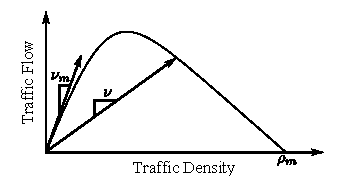
\includegraphics[height=3cm]{pics/d-q}\\
  \caption{Density-flow chart}
  \label{fig:d_q}
\end{figure}

Now, let $I(k)$ be the sum of the traffic densities that all vehicles meet at the instant $k$ in the network. For vehicles in the lane $i$, let $\rho_i(k)$ denote their traffic density at time $k$, $i\in \{1,\cdots,n\}$. Hence, we have
$$I(k)=\sum_{i=1}^{n} x_i(k)\rho_i(k)$$
Furthermore, since $\rho_i(k)=x_i(k)/h_i$ where $h_i$ is the length of the lane $i$, $i\in \{1,\cdots,n\}$, the sum of the traffic densities of all vehicles is finally restated as
\begin{equation}
\label{equ:quality_service}
I(k)=\sum_{i=1}^{n}
\frac{x_i(k)^2}{h_i}=\vec{x}(k)^T\mat{P}_h\vec{x}(k)
\end{equation}
where $\mat{P}_h$ is the diagonal matrix with the diagonal elements $1/h_i$. Since $x_i^*=\frac{h_i}{h_{veh}}$, where $h_{veh}$ is the average car length, it follows
\begin{equation}
I(k) = \sum_{i=1}^{n}\frac{x_i(k)^2}{h_{veh} x_i^*}
= \frac{2}{h_{veh}} \frac{1}{2}\vec{x}(k)^T\mat{P}\vec{x}(k)
= \frac{2}{h_{veh}} \psi(k)
\end{equation}

This indicates that the transportation entropy is proportional to the traffic densities $I(k)$ and hence it becomes now clear that this  transportation entropy  is an appropriate measurement of system disorder.
% It is also important to note that the entropy \eqref{equ:Tran_entropy} is a Lyapunov candidate function, which is very useful in control issues.

% \subsection{Dissipativity of Entropy}

% Though the second law of thermodynamics can not be applied in transportation context naturally, we still wonder whether it can be achieved in certain conditions. The major motive is that the transportation disorder corresponds to the thermodynamic order. If the transportation system has similar principle with the second law of thermodynamics, it will have the tendency to decrease its disorder and become better organized. More precisely, if the direction of the net traffic flow between any two transportation areas is from the more crowded one to the less crowded one as the energy does in the thermodynamic system, all congestions within the transportation network will tend to be evacuated.
% 
% Now, consider the anti-Clausius inequality \eqref{equ:anti_clausius} and its meaning in thermodynamic context, it can be stated that the idea is to achieve the phenomenon that the increase of the transportation entropy is always beneath its supply from the outside. In other words, the corresponding version of anti-Clausius inequality should be presented and verified.

Now, in transportation context, the input vehicles bring disorder to the system. This supplied disorder depends on not only the number of the input vehicles, but also the distribution of them. The vehicles which enter the more crowded lanes bring more disorder than the ones with same quantity which enter the less crowded lanes. Since the occupancies represent how the lanes are crowed, it is natural to measure the supplied entropy with respect to the input flows and the occupancy factors. Let $\vec{f}=[f_1,\cdots,f_n]^T$ be the vector of all occupancies. Note that because $\vec{f}(k)$ corresponds to the beginning of the interval $k$ while $\vec{f}(k+1)$ corresponds to the end of it, the supplied entropy in the interval $k$ should correspond to $\vec{f}(k+1)$ rather than $\vec{f}(k)$. So, we define
$$S(k)=\vec{f}(k+1)^T\vec{r}(k)$$
as the supplied entropy in the interval $k$. Furthermore, since $\vec{f}=\mat{P}_x\vec{x}$ in view of \eqref{equ:occupancy}, the supplied entropy is restated as
\begin{equation}\label{equ:supply}
    S(k)=\vec{x}(k+1)^T \mat{P} \vec{r}(k)
\end{equation}
Now, as in the anti-Clausius inequality \eqref{equ:anti_clausius}, we propose its corresponding version in transportation context as follows
\begin{equation}\label{equ:dissipative}
\psi(\vec{x}(k+1))-\psi(\vec{x}(k)) \leq S(k),\quad \forall
k\in\mathbb{N}
\end{equation}
If this inequality is verified, the transportation system has the tendency to decrease its disorder and become better organized.

Furthermore, according to the \citet{willems_dissipative_1972} and \citet{hill_dissipative_1980}, \eqref{equ:dissipative} also implies the dissipativity with the entropy \eqref{equ:Tran_entropy} as the storage function and with \eqref{equ:supply} as the supply function. In this case, \eqref{equ:dissipative} is called dissipation inequality. Figure \ref{fig:trans_dis} illustrates this dissipativity of system disorder. Indeed, the input flows bring disorder to the transportation system to make it worse organized. At the same time, the appropriate traffic signal control dissipates the traffic so that the system stores only a part of this input disorder.
\begin{figure}[ht]
  \centering
  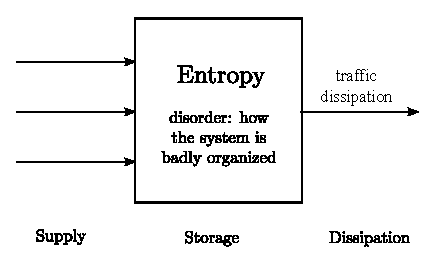
\includegraphics{pics/trans_dis}\\
  \caption{Dissipativity of transportation entropy}
  \label{fig:trans_dis}
\end{figure}

This dissipativity implies that the storage of the system disorder is always smaller than or equal to the supplied one from the outside. In other words, if this dissipative phenomenon exists in the transportation system, the system disorder will tend to decrease and hence the system will tend to become better organized.

This dissipativity does not exist naturally. But, it is known that the traffic signals have the ability to control the traffic flows. Therefore, it is possible that under certain control schemes, the traffic signals can verify the dissipation inequality \eqref{equ:dissipative}. This inequality can be considered as one of objectives for traffic signal control.

\section{Nominal Situation and Occupancy Equilibrium}\label{sec:nominal}

In the researches about thermodynamic systems, the closed system, which has no exchange with the environment, is one of the most studied subjects. Indeed, the closed thermodynamic system has special features. For example, in any closed thermodynamic system, the ectropy (resp, entropy) keeps decreasing (resp, increasing) until reaching the equilibrium state when all connected subsystems have the same temperature. The equilibrium also corresponds to the minimal possible ectropy and maximal possible entropy. Since the ectropy is a Lyapunov function, the closed thermodynamic system is Lyapunov stable \citep{haddad_thermodynamic_2005}.

Unfortunately, the transportation system is always open. Indeed, the openness is imposed by the transportation functionality. However, there exists a nominal situation \citep{diakaki_multivariable_2002} in the transportation network which has some common features with the closed thermodynamic system. The nominal situation means that with certain traffic demands and certain traffic signal settings, the input vehicles equals the output vehicles for each traffic lane, in other words, the queue lengths of all traffic lanes keep constant. In this paper, these certain traffic demands are called nominal inputs from the outside, denoted by
$$\vec{r}^N=\{r_1^N,\cdots,r_n^N\}$$
Obviously, in the nominal situation, the net exchange between the transportation system and the outside equals zero in each cycle, that means
\begin{equation}\label{equ:nominal_exchange}
Q(k)\equiv 0, \quad \forall k\in\mathbb{N}
\end{equation}

Since the transportation system is lossless with the storage function $U$ and the supply function $Q$, \eqref{equ:nominal_exchange} infers that the total amount of vehicles $U$ within the whole system keeps constant in the nominal situation. This is very similar with the closed thermodynamic system which has zero exchange of energy with the environment.
% Hence, we propose that the nominal situation of the transportation system can be analogized to the closed status of the thermodynamic system.

Note that \citet{de_oliveira_multi-agent_2010} have presented some effective procedures to estimate the nominal parameters for the general transportation system, hence it is reasonable to assume the availability of the nominal situation in general.

Now, define the disturbances of the transportation system as the difference between the real input flows and the nominal ones, which is given by
\begin{equation}
\vec{\omega}(k)\triangleq\vec{r}(k)-\vec{r}^N, \quad \forall
k\in\mathbb{N}
\end{equation}
Since the nominal situation of transportation system is similar to the closed status of thermodynamic system, the disturbances $\vec{\omega}$ are more appropriate than the input traffic flows $\vec{r}$ to present the input ``energy'' for the transportation system, specially when we consider the dissipativity phenomenon. Indeed, let
\begin{equation}\label{equ:supply_omega}
  S_\omega(k) = \vec{x}(k+1)^T \mat{P} \vec{\omega}(k)
\end{equation}
be the new supply function with respect to $\vec{\omega}$. Consequently, the dissipativity presented in previous section can be modified to the one with the entropy \eqref{equ:Tran_entropy} as the storage function and with \eqref{equ:supply_omega} as the supply function. This is stated in the following theorem.

\begin{thm}
If the transportation system described by the difference equation \eqref{equ:mdl_gnl} is dissipative with respect to the storage function \eqref{equ:Tran_entropy} and the supply function \eqref{equ:supply_omega}, then the system is also dissipative with respect to the same storage function and the supply function \eqref{equ:supply}.
\end{thm}
\begin{proof}
The dissipation inequality related with the storage function (\ref{equ:Tran_entropy}) and the supply function
(\ref{equ:supply_omega}) is
\begin{equation}\label{equ:dissipative_omega}
  \psi(\vec{x}(k+1))-\psi(\vec{x}(k)) \leq S_\omega(k)
\end{equation}
Since $\vec{\omega}(k)=\vec{r}(k)-\vec{r}^N$, it follows
\begin{align*}
S_\omega(k) &= \vec{x}(k+1)^T \mat{P} (\vec{r}(k)-\vec{r}^N)\\
    &= \vec{x}(k+1)^T \mat{P} \vec{r}(k)-\vec{x}(k+1)^T\mat{P}\vec{r}^N
\end{align*}
Since the nominal inputs and all queue lengths are non-negative, this infers
$$S_\omega(k)\leq \vec{x}(k+1)^T \mat{P} \vec{r}(k) = S(k)$$
So, the conclusion follows.
\end{proof}
% Now, the second law of thermodynamics corresponds to this new dissipativity.
This theorem also implies that the dissipativity with the supply function $S_\omega(k)$ is more strict than the one with the supply function $S(k)$. Hence, by taking the new dissipation inequality \eqref{equ:dissipative_omega} as the control objective, the traffic signal control can generate better performances.

Finally, we close this section by introducing the concept of thermal equilibrium into the transportation context. For a closed thermodynamic system, if a pair of connected subsystems have different temperatures, the energy transmission will emerge between them so that their temperatures tend to approximate. After enough time, all connected subsystems will have the same temperature so that no energy movement can emerge any more. In other words, the system loses all its capacity to do useful work in this moment. This particular state is called thermal equilibrium state \citep{cengel_thermodynamics:_2001}, which also corresponds to the maximal entropy and minimal ectropy in the closed thermodynamic system.

This concept of equilibrium can be also introduced into the transportation context to denote the state when the occupancies of all traffic lanes are the same. Mathematically, this occupancy equilibrium means
\begin{equation}\label{equ:equilibrium}
\frac{x_1}{x_1^*}=\cdots=\frac{x_n}{x_n^*}=\alpha
\end{equation}
where
$$\alpha = \frac{\vec{\epsilon}^T\vec{x}}{\vec{\epsilon}^T\vec{x}^*}
\in[0,1]$$
It is clear that, the occupancy equilibrium  implies that no particular concentration of vehicles exists in the system and hence the possibility to emerge congestion is extremely low. This observation is demonstrated in the following theorem.


% It can be easily proved that the transportation equilibrium
% corresponds to the minimization of the transportation entropy with
% certain amount of traffic.
% The relationship between the transportation equilibrium and the transportation entropy is stated in the following theorem.

\begin{thm}\label{thm:entropy_equilibrium}
Assume that the total amount of vehicles $N$ is given, the transportation entropy \eqref{equ:Tran_entropy} is minimized when the system reaches the equilibrium state \eqref{equ:equilibrium}.
\end{thm}
\begin{proof}
To minimize the entropy, consider the problem
\begin{align}\label{equ:pro_min_psi}
\min\; &\psi(\vec{x}) = \frac{1}{2}\vec{x}^T\mat{P}\vec{x}\\
s.t.\; &\sum_{i=1}^n x_i = N \nonumber
\end{align}
Since $\psi(\vec{x})$ is a convex function, by applying the method of Lagrange multipliers to solve the problem \eqref{equ:pro_min_psi}, we have the equivalent unconstrained problem:
$$\min J(\vec{x},\beta) =
\frac{1}{2}\vec{x}^T\mat{P}\vec{x}+\beta(\sum_{i=1}^n x_i - N)$$
whose solution can be obtained by solving the equations
\begin{align}
\label{equ:tmp_min_J_1}
\frac{\partial J}{\partial x_i} &= \frac{x_i}{x_i^*}+\beta =0,
i\in\{1,\cdots,n\}\\
\label{equ:tmp_min_J_2}
\frac{\partial J}{\partial \beta} &= \sum_{i=1}^n x_i - N =0
\end{align}
Now, from \eqref{equ:tmp_min_J_1}, we have
$$\frac{x_1}{x_1^*}=\cdots=\frac{x_n}{x_n^*}=-\beta
$$
Apparently, $\beta$ can only equal to $-\alpha$, which completes the proof.
\end{proof}

It follows immediately from the this theorem that the occupancy equilibrium leads to the minimal disorder in the network. Hence, the occupancy equilibrium is actually the ideal state for the transportation network and the principal objective shared by all dynamic traffic signal control strategies.

\section{Conclusion}

This paper has presented a novel thermodynamic point of view for the transportation system. Indeed, the comparison between thermodynamic systems and transportation systems has shown that they are very similar by regarding the vehicles as the energy and regarding the traffic lanes as the thermodynamic subsystems. In addition, the concepts of thermal capacity and temperature are also introduced into transportation context to correspond to lane capacity and occupancy respectively. Based on the correspondence of concepts, it has been demonstrated that the first law of thermodynamics corresponds to the conservation of vehicles. Then, for introducing the notion of entropy, it has been shown that the significations of order in transportation context and thermodynamic one is opposite. Hence, the transportation entropy is defined according to the thermodynamic ectropy that measures the order of thermodynamic systems. The transportation entropy has been proved to be proportional to the traffic densities and hence it is an appropriate measurement of system disorder.
% Hence, this paper was able to introduce the thermodynamic concepts into the transportation context. In particular, it has been demonstrated that the transportation system can have a similar notion of the entropy to measure the system disorder.
In addition, by taking the transportation entropy as the storage function, certain dissipativity phenomenon has been presented to reduce the disorder and render the system better organized. The existence of this dissipativity depends on the traffic signals, hence it can be considered as one of objectives for designing control strategies.
% Though this phenomenon doesn't exist naturally, it can be used as the objective for traffic signal control.
Furthermore, since temperature corresponds to occupancy, thermal equilibrium can be introduced into transportation context to represent the state when all traffic lanes share the same occupancy. It has been proven that the transportation entropy minimizes when the system reaches the occupancy equilibrium. Finally, though transportation network is always open, this paper has also shown that the nominal situation in transportation systems is similar with the closed status in thermodynamic ones.

By bring certain thermodynamic concepts and principles into transportation context, the work in this paper provides a completely new approach to get the view of transportation network. The results can be further applied to analyze the system performances and design traffic signal control strategies.

\bibliographystyle{model5-names}
\bibliography{zhou_refs}

\end{document}
